% \documentclass[aspectratio=169, 11pt]{beamer}
\documentclass[aspectratio=169, 11pt, handout]{beamer}

% ── Theme ──
\usetheme{Madrid}
\usecolortheme{default}
\setbeamertemplate{navigation symbols}{}
\setbeamertemplate{footline}{%
  \leavevmode\hbox{%
    \begin{beamercolorbox}[wd=.333333\paperwidth,ht=2.5ex,dp=1ex,center]{author in head/foot}%
      \usebeamerfont{author in head/foot}\insertshortauthor
    \end{beamercolorbox}%
    \begin{beamercolorbox}[wd=.333333\paperwidth,ht=2.5ex,dp=1ex,center]{title in head/foot}%
      \usebeamerfont{title in head/foot}\insertshorttitle
    \end{beamercolorbox}%
    \begin{beamercolorbox}[wd=.333333\paperwidth,ht=2.5ex,dp=1ex,right]{date in head/foot}%
      \usebeamerfont{date in head/foot}\insertframenumber{} / \inserttotalframenumber\hspace*{2ex}
    \end{beamercolorbox}}}

% ── Packages ──
\usepackage{amsmath,amssymb}
\usepackage{booktabs}
\usepackage{xcolor}
\usepackage{colortbl}
\usepackage{graphicx}
\usepackage{tikz}
\usetikzlibrary{arrows.meta, positioning, calc}

% ── Colors ──
\definecolor{sbgreen}{HTML}{00704A}  % course accent
\definecolor{warnred}{HTML}{CC0000}
\definecolor{noteblue}{HTML}{2060A0}

% ── Commands ──
\newcommand{\E}{\mathbb{E}}
\newcommand{\Var}{\mathrm{Var}}
\newcommand{\Cov}{\mathrm{Cov}}
\newcommand{\SE}{\mathrm{SE}}
\newcommand{\Prob}{\mathrm{Pr}}
\newcommand{\indep}{\perp\!\!\!\perp}

\usepackage{soul}
\newcommand{\NUM}[2]{\sethlcolor{yellow}\hl{#1\,\textsuperscript{?}}\marginpar{\tiny #2}}
% Beamer frames are typeset inside boxes, where \marginpar raises "Not in outer par mode"
% and \marginparwidth is 4pt. Same marker; the provenance note goes to the frame footnote.
\renewcommand{\NUM}[2]{\sethlcolor{yellow}\hl{#1\,\textsuperscript{?}}\footnote[frame]{\tiny #2}}
% Compact footnote layout so several provenance notes fit under one frame.
\setbeamertemplate{footnote}{\noindent\raggedright\hspace*{0.6em}\tiny\insertfootnotemark\,\insertfootnotetext\par}

% Version 2 (2026-09-29). Course spine: estimand -> identification -> estimation.
% Changes from slides.tex: m07/CHANGES-v2.md.
\newcommand{\spinestep}[1]{\textcolor{sbgreen}{\textbf{#1}}}

% ── Title ──
\title[Meeting 7]{Meeting 7: When the Logs Must Answer}
\subtitle{Applied Causal Inference for Business}
\author{Zhikun Lu}
\date{\today}

\begin{document}

% ====================================================================
\begin{frame}
\titlepage
\end{frame}

% ====================================================================
\begin{frame}{Where Does the Counterfactual Come From?}

\begin{center}
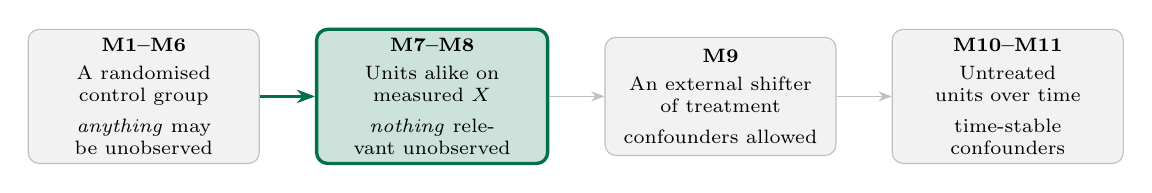
\begin{tikzpicture}[
    node distance=0.45cm and 0.7cm,
    box/.style={draw, rounded corners, minimum width=2.9cm, minimum height=1.5cm,
                font=\scriptsize, align=center, text width=2.7cm},
    active/.style={box, fill=sbgreen!20, draw=sbgreen, very thick},
    inactive/.style={box, fill=gray!10, draw=gray!50}
]
\node[inactive] (A) {\textbf{M1--M6}\\[2pt] A randomised control group\\[3pt] \emph{anything} may be unobserved};
\node[active, right=of A] (B) {\textbf{M7--M8}\\[2pt] Units alike on measured $X$\\[3pt] \emph{nothing} relevant unobserved};
\node[inactive, right=of B] (C) {\textbf{M9}\\[2pt] An external shifter of treatment\\[3pt] confounders allowed};
\node[inactive, right=of C] (D) {\textbf{M10--M11}\\[2pt] Untreated units over time\\[3pt] time-stable confounders};

\draw[-{Stealth}, thick, sbgreen] (A) -- (B);
\draw[-{Stealth}, gray!50] (B) -- (C);
\draw[-{Stealth}, gray!50] (C) -- (D);
\end{tikzpicture}
\end{center}

\bigskip

\begin{center}
\small Until today the control group was \emph{given} to us. Today nobody randomised anything.\\
We must build the comparison from the records the assignment rule left behind.
\end{center}
\end{frame}

% ====================================================================
\begin{frame}{Today's Plan}

\begin{center}
\small
\begin{tabular}{rp{11.6cm}}
\toprule
\textbf{Minutes} & \\
\midrule
0--15 & \textbf{Reading and critique C4} --- on paper, no devices \\
15--50 & \spinestep{Estimand:} the programme as it ran. \spinestep{Identification:} the engine's rule is the assignment mechanism; what must be true for logs to stand in for an experiment \\
60--110 & Choosing controls. \spinestep{Design before analysis}, then \spinestep{estimation} at scale: three adjustments and whom each describes \\
120--180 & \textbf{Twelve proposal presentations} \\
\bottomrule
\end{tabular}
\end{center}

\bigskip

\textbf{Case:} Lin's coupon programme, Meeting 7 (Releases 1--5). \quad \textbf{After class:} the take-home adjustment core --- the Rivergate control audit (30--45 min), with Notebook 7.

\bigskip

\textbf{Reading:} technical notes for Meeting 7, including AIPW and double robustness on the Rivergate numbers (Section 3).
\end{frame}

% ====================================================================
\begin{frame}{Critique C4: Five Questions, Every Time}

Read the one-page case silently. Notes on your own, then pairs, then the room.

\bigskip

\begin{enumerate}
    \item What is the claim?
    \item What causal question does the decision need?
    \item Who is the comparison group?
    \item What else could produce this pattern? Give the mechanism and the \textbf{direction} of the bias.
    \item What would you do to find out?
\end{enumerate}

\bigskip

\small Not every report is flawed. If this one is sound, say \emph{why} --- and name what it still cannot tell the decision-maker. Hand in your notes at minute 15.
\end{frame}

% ====================================================================
\section{The Estimand: The Programme as It Ran}
% ====================================================================

% [RELEASE R1 — narrative: the programme, the CFO's position, the sales reading]
\begin{frame}{The Coffee Chain, After the Experiment}

\textbf{Lin} runs customer analytics. In Q2 the chain ran the coupon experiment you analysed in M1--M6. Its \textbf{campaign engine} (M5) turned the results into a targeting rule.

\bigskip

In Q3 the engine's rule went live: a \textyen 10 coupon to \textbf{40\%} of the loyalty base, chosen by a \textbf{scoring rule} on recency, tier and spend, throttled by a daily contact cap.

\bigskip
\pause

\textbf{Now the CFO wants the programme reviewed.} Sales has pulled the Q3 logs:

\begin{center}
\small
\begin{tabular}{lrr}
\toprule
& \textbf{Got coupon} & \textbf{No coupon} \\
\midrule
Purchase rate & 0.40 & 0.62 \\
\bottomrule
\end{tabular}
\end{center}

\smallskip
\begin{center}
Sales' reading: \emph{``The coupon repels customers. Kill it.''}
\end{center}

\bigskip

\textbf{And the CFO will not fund another experiment.} The Q3 logs must answer.
\end{frame}

% ====================================================================
\begin{frame}{The Number That Decides It}

A purchase earns \textyen 30 of margin. The coupon costs \textyen 10, paid on \emph{every} purchase a coupon holder makes.

\bigskip

Per coupon sent to last quarter's recipients:
\[
\text{net} \;=\; \underbrace{\tau \times 30}_{\text{purchases the coupon caused}} \;-\; \underbrace{10 \times 0.40}_{\text{coupons redeemed}} .
\]

\bigskip
\pause

\begin{alertblock}{Break-even lift}
\[
\tau^{*} \;=\; \frac{10 \times 0.40}{30} \;=\; \frac{4}{30} \;=\; \mathbf{0.133}
\]
\end{alertblock}

\bigskip

Sales' number is $-0.22$. Every estimate today is a lift. The only question is \textbf{which side of $0.133$} it lands on.
\end{frame}

% ====================================================================
\begin{frame}{Three Steps for the Logs}

\begin{center}
\small
\begin{tabular}{p{2.8cm}p{9.8cm}}
\toprule
\spinestep{Estimand} & The effect of the coupon \textbf{on the members who got it}, as the programme ran: the ATT, held against $0.133$. \\[0.5em]
\spinestep{Identification} & No coin this time. The \textbf{assignment mechanism is the engine's rule}: we must argue that, among members the rule saw as identical, who got a coupon was as good as random --- and that the rule left something to chance. \\[0.5em]
\spinestep{Estimation} & First an \textbf{outcome-free design stage}: reconstruct the rule, check overlap, fix the estimand. Only then open the purchases: standardisation, weighting. \\
\bottomrule
\end{tabular}
\end{center}

\bigskip

The same system that made the decisions in M5 is what we must now adjust for. An automated decision-maker does not remove confounding; it \emph{writes it down}.
\end{frame}

% ====================================================================
% [RELEASE R2 — two-segment table; worksheet attempt before the next frame]
\begin{frame}{Two Kinds of Customer}

The scoring rule mostly sent coupons to \textbf{lapsed} customers --- the ones M5 told you to target.

\bigskip

\begin{center}
\small
\begin{tabular}{lrrrrr}
\toprule
\textbf{Segment} & \textbf{$n$} & \textbf{Coupon share} & \textbf{Treated} & \textbf{Control} & \textbf{Purchase rate (T / C)} \\
\midrule
Active & 500 & 0.20 & 100 & 400 & 0.80 / 0.75 \\
Lapsed & 500 & 0.80 & 400 & 100 & 0.30 / 0.10 \\
\bottomrule
\end{tabular}
\end{center}

\bigskip

\textbf{In pairs:} compute the overall purchase rate in each arm, then the difference within each segment. Commit in writing --- does the CFO kill the programme?
\end{frame}

% ====================================================================
\begin{frame}{Pooled, Then Within Segment}

\[
\bar Y_{\text{T}} = \frac{100(0.80) + 400(0.30)}{500} = 0.40, \qquad
\bar Y_{\text{C}} = \frac{400(0.75) + 100(0.10)}{500} = 0.62
\]
\vspace{-1.2em}
\[
\text{difference} = \textcolor{warnred}{-0.22}
\]

\pause
\medskip

Within each segment the coupon \textbf{raises} purchases:

\begin{center}
\small
\begin{tabular}{lrr}
\toprule
& \textbf{Active} & \textbf{Lapsed} \\
\midrule
Treated $-$ control & $0.80 - 0.75 = \textcolor{sbgreen}{+0.05}$ & $0.30 - 0.10 = \textcolor{sbgreen}{+0.20}$ \\
\bottomrule
\end{tabular}
\end{center}

\pause
\medskip

The pooled number decomposes exactly as in M1. Recipients are $0.2$ active, $0.8$ lapsed:
\vspace{-0.4em}
\begin{align*}
\text{ATT} &= 0.2(0.05) + 0.8(0.20) = 0.17 \\
\text{selection bias} &= \E[Y(0) \mid D{=}1] - \E[Y(0) \mid D{=}0] = 0.23 - 0.62 = -0.39 \\
\text{naive} &= 0.17 - 0.39 = \textcolor{warnred}{-0.22}
\end{align*}
\vspace{-1.0em}

Same logs. Opposite sign. The recipients were chosen \emph{because} they were unlikely to buy.
\end{frame}

% ====================================================================
% [REVISED: potential-outcome statement first; OVB as intuition]
\begin{frame}{Confounding by the Targeting Rule}

The rule sends coupons to customers whose baseline purchase rate is low.

\begin{center}
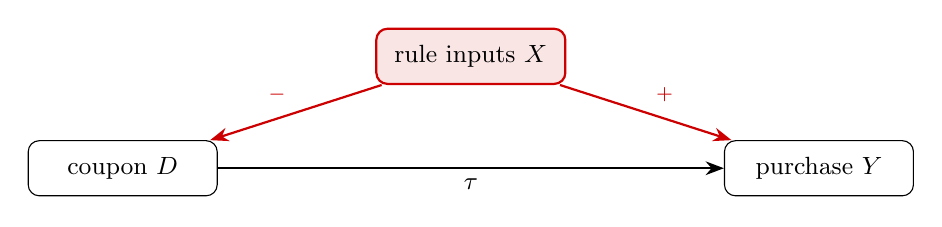
\begin{tikzpicture}[
    node distance=0.7cm and 2.0cm,
    v/.style={draw, rounded corners, minimum width=2.4cm, minimum height=0.7cm, font=\small},
    hid/.style={v, fill=warnred!10, draw=warnred, thick}
]
\node[hid] (X) {rule inputs $X$};
\node[v, below left=of X] (D) {coupon $D$};
\node[v, below right=of X] (Y) {purchase $Y$};
\draw[-{Stealth}, warnred, thick] (X) -- node[above left, font=\scriptsize] {$-$} (D);
\draw[-{Stealth}, warnred, thick] (X) -- node[above right, font=\scriptsize] {$+$} (Y);
\draw[-{Stealth}, thick] (D) -- node[below, font=\small] {$\tau$} (Y);
\end{tikzpicture}
\end{center}

\textbf{In potential outcomes} (M1): the bias is $\E[Y(0) \mid D = 1] - \E[Y(0) \mid D = 0] = 0.23 - 0.62 = -0.39$. The rule picked members who would \emph{not} have bought anyway.

\pause

\medskip

\textbf{The same thing in regression language}, as intuition: leaving the rule's input $X$ out of $Y = \alpha + \tau D + \gamma X + \varepsilon$ adds $\gamma \cdot \Cov(D, X)/\Var(D)$. Here $\gamma > 0$ (the active buy more) and $\Cov(D, X) < 0$ (the rule avoids them): negative, large enough to flip the sign.

\medskip

\textbf{Both arrows are the rule's doing --- and the rule is written down.}
\end{frame}

% ====================================================================
\begin{frame}{Why Not Just Run Another Experiment?}

Because the CFO said no --- and because that answer is the normal one.

\bigskip

\begin{center}
\small
\begin{tabular}{lll}
\toprule
\textbf{Situation} & \textbf{Why no experiment} & \textbf{What exists instead} \\
\midrule
This coupon programme & budget; a live rule already in place & the rule's logs \\
A retailer's pricing & prices set by a system, not assignable & the system's logs \\
A platform's ranking & hosts set prices; platform only suggests & observational listings \\
A drug already prescribed & ethics; the treatment is standard care & clinical records \\
\bottomrule
\end{tabular}
\end{center}

\bigskip
\pause

In each case a \textbf{rule} assigned the treatment from things it observed. The question is never ``can we randomise?'' but

\begin{center}
\emph{do we know what the rule looked at, and did it leave anything to chance?}
\end{center}
\end{frame}

% ====================================================================
\section{Identification: The Rule Is the Assignment Mechanism}
% ====================================================================

\begin{frame}{What Must Be True}

\begin{alertblock}{Identifying assumption: conditional exchangeability}
Among customers the rule saw as identical, who got the coupon is as good as random:
\[
\{Y(0), Y(1)\} \;\indep\; D \;\mid\; X .
\]
\end{alertblock}

\bigskip
\pause

Two more, less dramatic but not optional:

\begin{itemize}
    \item \textbf{Overlap.} $0 < \Prob(D = 1 \mid X = x) < 1$ for every $x$ we report on. Some coupons, some non-coupons, in every cell.
    \medskip
    \item \textbf{Consistency.} $Y = Y(D)$: one coupon, delivered the same way to everyone; my coupon does not change your purchase.
\end{itemize}

\bigskip

Randomisation in M1 bought the first two for free. Today we must \textbf{argue} for them from the case.
\end{frame}

% ====================================================================
\begin{frame}{The Assumptions, Sentence by Sentence}

From Lin's description of the Q3 programme:

\bigskip

\begin{center}
\small
\begin{tabular}{p{6.4cm}p{6.6cm}}
\toprule
\textbf{The case says} & \textbf{Which buys} \\
\midrule
``Coupons were assigned by the scoring rule and by nothing else.'' & Exchangeability: no one hand-picked recipients on something unrecorded. \\[0.5em]
``Every field the rule read is in the export.'' & Exchangeability: $X$ contains the rule's inputs. \\[0.5em]
``The daily cap meant no score band was sent coupons on every day.'' & Overlap: within a band, some got it and some did not. \\[0.5em]
``One coupon design, one channel, one redemption rule.'' & Consistency. \\
\bottomrule
\end{tabular}
\end{center}

\bigskip
\pause

\textbf{Hold onto the first sentence.} We will test whether it is true before the hour ends.
\end{frame}

% ====================================================================
\begin{frame}{Standardisation}

If exchangeability holds \emph{within} cells of $X$, then within each cell the treated--control difference is a causal effect, and we combine cells by their population weights.

\begin{block}{Standardisation (the g-formula, Robins 1986)}
\[
\E[Y(1) - Y(0)] \;=\; \sum_x \Prob(X = x)\,\Bigl\{\E[Y \mid D = 1, X = x] - \E[Y \mid D = 0, X = x]\Bigr\}
\]
\end{block}

\pause
\medskip

\textbf{On the two segments:}
\[
\widehat\tau_{\text{ATE}} = 0.5 \times 0.05 + 0.5 \times 0.20 = \textcolor{sbgreen}{0.125}
\]

\medskip

Each within-cell difference needs \textbf{both arms present} in the cell --- that is where overlap enters, not as decoration.

\medskip

\textbf{Two functions to learn at scale:} $\mu_1(x) = \E[Y \mid D=1, x]$ and $\mu_0(x) = \E[Y \mid D=0, x]$. That is the T-learner of M3, now doing identification rather than targeting.
\end{frame}

% ====================================================================
\begin{frame}{Which Average Does the CFO Need?}

The same cell effects, three ways of weighting them (your warm-up):

\begin{center}
\small
\begin{tabular}{llrr}
\toprule
\textbf{Estimand} & \textbf{Weights} & \textbf{Value} & \textbf{Answers} \\
\midrule
ATE & population: $0.5 / 0.5$ & $0.125$ & ``coupon everyone?'' \\
ATT & who got coupons: $0.2 / 0.8$ & $\mathbf{0.17}$ & ``keep the programme as run?'' \\
ATU & who did not: $0.8 / 0.2$ & $0.08$ & ``extend to the rest?'' \\
\bottomrule
\end{tabular}
\end{center}

\pause
\medskip

The CFO's question is the second one. Against the break-even:
\[
\text{ATT} = 0.17 > 0.133 \quad\Longrightarrow\quad \text{net} = 0.17 \times 30 - 4 = \textcolor{sbgreen}{+\text{\textyen}1.1 \text{ per coupon}} .
\]

\medskip

Extending to everyone would use the ATE against a \emph{different} break-even, because everyone redeems more: $\E[Y(1)] = 0.55$, so $\tau^{*} = 5.5/30 = 0.183 > 0.125$. \textcolor{warnred}{Loses money.}

\medskip
\begin{center}
\textbf{Say which average you estimated, and for whom.}
\end{center}
\end{frame}

% ====================================================================
\section{Identification: Choosing Controls}
% ====================================================================

\begin{frame}{The DAG for the Logs}

Everything the rule read is a candidate control. Not everything in the export is.

\vspace{-0.3em}
\begin{center}
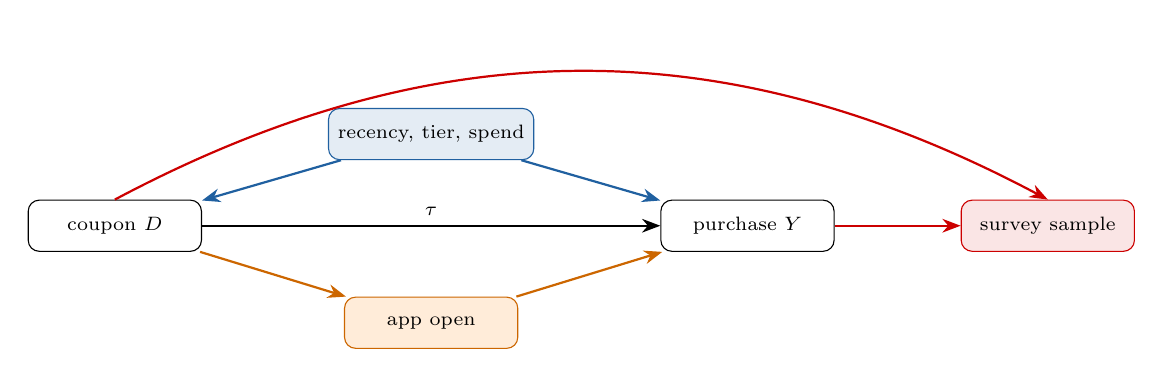
\begin{tikzpicture}[
    node distance=0.5cm and 1.6cm,
    v/.style={draw, rounded corners, minimum width=2.2cm, minimum height=0.65cm, font=\scriptsize},
    conf/.style={v, fill=noteblue!12, draw=noteblue},
    med/.style={v, fill=orange!15, draw=orange!80!black},
    col/.style={v, fill=warnred!10, draw=warnred},
    a/.style={-{Stealth}, thick}
]
\node[conf] (X) {recency, tier, spend};
\node[v, below left=of X] (D) {coupon $D$};
\node[v, below right=of X] (Y) {purchase $Y$};
\node[med, below=0.9cm of $(D)!0.5!(Y)$] (M) {app open};
\node[col, right=of Y] (S) {survey sample};
\draw[a, noteblue] (X) -- (D);
\draw[a, noteblue] (X) -- (Y);
\draw[a] (D) -- node[above, font=\scriptsize] {$\tau$} (Y);
\draw[a, orange!80!black] (D) -- (M);
\draw[a, orange!80!black] (M) -- (Y);
\draw[a, warnred] (D.north) to[bend left=28] (S.north);
\draw[a, warnred] (Y) -- (S);
\end{tikzpicture}
\end{center}

\medskip
\pause

\textbf{Blue:} the rule's inputs open the back door $D \leftarrow X \rightarrow Y$. Condition on them.

\textbf{Orange:} the app open is \emph{how} the coupon works. Condition on it and you block the effect.

\textbf{Red:} the survey went to coupon recipients \emph{and} recent purchasers. Condition on it and you \emph{create} a path.
\end{frame}

% ====================================================================
\begin{frame}{Good Controls and Bad Controls}
\begin{figure}
    \centering
    
\includegraphics[width=.95\linewidth]{fig/controls.png}
    % \caption{Enter Caption}
    \label{fig:controls}
\end{figure}
\end{frame}

% ====================================================================
\begin{frame}{Good Controls and Bad Controls}

Not every column in the export belongs in $X$. Including the wrong ones \textbf{introduces new bias}.

\bigskip

\begin{center}
\footnotesize
\begin{tabular}{llcl}
\toprule
\textbf{Column} & \textbf{Type} & \textbf{Include?} & \textbf{Why} \\
\midrule
Recency, tier, past spend & Confounder & \textcolor{sbgreen}{Yes} & Rule inputs that also predict buying \\
App open in coupon week & Mediator & \textcolor{warnred}{No} & Coupon $\to$ open $\to$ purchase \\
Redeemed the coupon & Post-treatment & \textcolor{warnred}{No} & A version of the outcome \\
In the Q3 survey sample & Collider & \textcolor{warnred}{No} & Sampled on coupon \emph{and} purchase \\
Store of first visit & Pre-treatment, not an input & Optional & Harmless; tightens the interval \\
\bottomrule
\end{tabular}
\end{center}

\bigskip
\pause

The test is not ``is it correlated with $Y$?'' --- the mediator and the collider both are. The test is \textbf{when} the column was determined, and \textbf{by what}. Timing is necessary, not sufficient: a variable fixed \emph{before} the coupon can still be a collider if two unrecorded causes of $D$ and $Y$ both drive it.
\end{frame}

% ====================================================================
% [RELEASE R3 — collider worksheet; answer on the next frame after the attempt]
\begin{frame}{Exercise: The App-Open Column}

A junior analyst argues: ``Customers who never open the app cannot see the coupon. Restrict to app openers --- it makes the comparison fairer.''

\bigskip

Take a clean case: 1{,}000 customers, coupon \textbf{randomised} 50/50, and suppose the coupon has \textbf{no effect at all}.

\begin{itemize}
    \item Half the customers have \emph{high intent} and buy regardless; half have low intent and never buy.
    \item A customer opens the app if they received a coupon \textbf{or} have high intent.
\end{itemize}

\bigskip

\begin{center}
\small
\begin{tabular}{lrrr}
\toprule
& \textbf{$n$} & \textbf{Open the app} & \textbf{Buy} \\
\midrule
Coupon, high intent & 250 & 250 & 250 \\
Coupon, low intent  & 250 & 250 & 0 \\
No coupon, high intent & 250 & 250 & 250 \\
No coupon, low intent  & 250 & 0 & 0 \\
\bottomrule
\end{tabular}
\end{center}

\medskip
\textbf{In pairs:} the coupon effect \emph{among app openers}. Commit before the next frame.
\end{frame}

% ====================================================================
\begin{frame}{The App-Open Answer}

Among app openers:
\[
\Prob(\text{buy} \mid \text{coupon, open}) = \frac{250}{500} = 0.50, \qquad
\Prob(\text{buy} \mid \text{no coupon, open}) = \frac{250}{250} = 1.00 .
\]

\bigskip

\begin{center}
\Large ``Effect'' $= \textcolor{warnred}{-0.50}$ \qquad for a true effect of $\mathbf{0}$.
\end{center}

\bigskip
\pause

The coupon was randomised, so there was \textbf{no confounding to fix}. Restricting to openers selected \emph{all} treated customers but only the \emph{high-intent} untreated ones. Conditioning on a variable that both $D$ and intent cause makes $D$ and intent dependent.

\bigskip

\begin{alertblock}{The pattern}
A variable determined \emph{after} treatment, by treatment and by the outcome's causes, is a collider. ``Fairer comparison'' arguments almost always propose one.
\end{alertblock}
\end{frame}

% ====================================================================
\begin{frame}{Is Exchangeability Credible?}

Once the controls are the rule's inputs, exchangeability says: among customers with the same inputs, who got the coupon was down to the cap and the calendar. Substantive and \textbf{untestable}.

\begin{center}
\small
\begin{tabular}{lll}
\toprule
\textbf{Could have moved both $D$ and $Y$} & \textbf{In the export?} & \textbf{Status} \\
\midrule
Recency, tier, past spend & \textcolor{sbgreen}{Yes} & Controlled for \\
Score band, contact-cap day & \textcolor{sbgreen}{Yes} & Controlled for \\
Store-manager ``VIP'' additions & \textcolor{warnred}{No} & Residual confounding, if they exist \\
A regional push in week 9 & \textcolor{warnred}{Unclear} & Ask Lin \\
\bottomrule
\end{tabular}
\end{center}

\bigskip
\pause

\textbf{Professional standard:} state the assumption, list what the rule saw, list what it might have seen that you cannot, and say how large that would have to be to matter (M8 shows how to price it).

\medskip
\textbf{Rivergate worksheet:} the same audit on a second firm's logs, for the take-home core.
\end{frame}

% ====================================================================
\section{Design, Then Estimation at Scale}
% ====================================================================

% [RELEASE R4 — full export description; collect three proposed estimators on the board]
\begin{frame}{The Real Logs}

\begin{center}
\small
\begin{tabular}{lr}
\toprule
Customers in the Q3 export & \NUM{40{,}000}{sim coupon-logs v1: number of loyalty customers in the export} \\
Received the coupon & \NUM{16{,}100}{sim coupon-logs v1: treated count} \\
Recorded fields the rule read & \NUM{14}{sim coupon-logs v1: rule inputs} \\
Purchase rate, coupon / no coupon & \NUM{0.41}{sim coupon-logs v1: treated purchase rate} / \NUM{0.60}{sim coupon-logs v1: control purchase rate} \\
\bottomrule
\end{tabular}
\end{center}

\bigskip
\pause

The rule is \textbf{banded}: a score from the 14 fields, cut into bands; each band had a daily send probability, throttled by the cap.

\begin{itemize}\small
    \item the top band was sent coupons on almost every day; the bottom band almost never
    \item bands in the middle were sent on some days and not others
\end{itemize}

\bigskip

\textbf{In pairs:} write down the model you would fit. Three proposals go on the board.
\vspace{1.2em}
\end{frame}

% ====================================================================
\begin{frame}{Design Before Analysis}

The purchase column stays \textbf{locked}. Using only the 14 fields and the coupon column:

\begin{enumerate}
    \item \textbf{Reconstruct the assignment mechanism.} Fit the coupon on the rule's inputs: $\hat e(x)$ is the band's send probability, throttled by the cap.
    \item \textbf{Check overlap, band by band.} Where is $\hat e(x)$ near 0 or 1? Who has no comparison?
    \item \textbf{Fix the estimand and the trimming rule.} If some bands must go, the estimand becomes the ATT \emph{on the rest} --- decided now, in writing.
    \item \textbf{Check balance} of the 14 fields after weighting.
\end{enumerate}

\bigskip

\begin{block}{Why before}
Every choice above can be made without an outcome. Made after, each one could be tuned to the answer --- the same reason M4 froze the partition and M5 froze the list (Rubin: \emph{design before analysis}).
\end{block}
\end{frame}

% ====================================================================
\begin{frame}{Predict Before You Look}

Two segments worked by hand. The export has 14 fields and a banded rule.

\bigskip

\textbf{In pairs, write down three numbers} --- the estimated lift:

\bigskip

\begin{enumerate}
    \item with no controls
    \item regressing purchase on coupon and the 14 fields, linearly
    \item reweighting each customer by the inverse of their coupon probability
\end{enumerate}

\bigskip

Against the break-even \NUM{0.14}{p1-hat / 3, p1-hat = treated purchase rate in the sim export}, which ones keep the programme?

\bigskip

\begin{center}
\small Commit before the next slide.
\end{center}
\end{frame}

% ====================================================================
% [RELEASE R5 — the ladder; reveal only after predictions are on the board]
\begin{frame}{The Ladder}

\begin{center}
\begin{tabular}{lr}
\toprule
\textbf{Comparison} & \textbf{Lift} \\
\midrule
Pooled, no controls & \NUM{$-0.19$}{sim coupon-logs v1: difference in means} \\
Linear regression on coupon and 14 fields & \NUM{$+0.06$}{sim coupon-logs v1: OLS coefficient on D with linear controls} \\
Standardisation, flexible outcome models & \NUM{$+0.14$}{sim coupon-logs v1: T-learner g-formula, ATT weights} \\
IPW, all customers & \NUM{$+0.10$}{sim coupon-logs v1: Hájek ATT estimator, untrimmed} \\
\midrule
\textit{(today's destination)} & \textcolor{sbgreen}{\NUM{$+0.16$}{sim coupon-logs v1: Hájek ATT, ê trimmed to [0.05, 0.95]}} \\
\bottomrule
\end{tabular}
\end{center}

\medskip
\pause

\begin{itemize}
    \item Adding the fields linearly recovers the \textbf{sign} and less than half the \textbf{magnitude}.
    \item Two methods that both ``adjust for $X$'' disagree by more than the break-even margin.
\end{itemize}

\begin{center}
\textbf{So: what does each one actually compute?}
\end{center}
\end{frame}

% ====================================================================
\begin{frame}{Attempt 1 --- Regression Adjustment}

\[
Y_i = \alpha + \tau D_i + X_i'\beta + \varepsilon_i
\]

\bigskip
\pause

\begin{center}
\Large $\widehat\tau = $ \NUM{$+0.06$}{sim coupon-logs v1: OLS on D and linear X} \qquad $\Longrightarrow$ \qquad \textcolor{warnred}{\textbf{kill}}
\end{center}

\bigskip
\pause

\textbf{Why it fails.} Two things at once.

\begin{itemize}
    \item The rule is a \emph{staircase} in the score; a linear term is a \emph{ramp}. Whatever the ramp misses stays in $\varepsilon$ and keeps confounding $\tau$.
    \item Even with the right controls, one coefficient on $D$ forces a \textbf{single} effect. When effects differ by segment (they do: $0.05$ vs $0.20$), OLS returns a weighted average that over-weights cells where the rule was \emph{least} decided --- not the ATT the CFO asked for.
\end{itemize}

\bigskip
\begin{center}
\small The second point is the M8 story in binary clothing; the notes state it. Today: a well-specified outcome model is not one line.
\end{center}
\end{frame}

% ====================================================================
\begin{frame}{Attempt 2 --- Standardisation With a Flexible Outcome Model}

Fit $\widehat\mu_1(x)$ on the coupon rows and $\widehat\mu_0(x)$ on the others with a boosted model. Then, for the recipients,
\[
\widehat\tau_{\text{ATT}} = \frac{1}{n_1}\sum_{i : D_i = 1} \bigl\{ Y_i - \widehat\mu_0(X_i) \bigr\} .
\]

\bigskip
\pause

\begin{center}
\Large $\widehat\tau = $ \NUM{$+0.14$}{sim coupon-logs v1: T-learner standardisation, ATT} \qquad $\Longrightarrow$ \qquad \textcolor{warnred}{\textbf{knife edge}}
\end{center}

\bigskip
\pause

\textbf{Where it strains.} $\widehat\mu_0(x)$ must be evaluated at recipients' $x$. For the top score band there are \NUM{31}{sim coupon-logs v1: control rows in the top band} untreated customers to learn from among \NUM{4{,}900}{sim coupon-logs v1: rows in the top band}. The model \emph{extrapolates} into that band, and nothing in the fit says so.

\bigskip

The estimate is honest about the middle bands and a guess about the top one. We need a method that \textbf{shows} us where the comparison is thin.
\end{frame}

% ====================================================================
\begin{frame}{The Old Decision Rule Is the Propensity Score}

\begin{block}{Propensity score}
$e(x) = \Prob(D = 1 \mid X = x)$: the probability the rule sent a coupon to a customer with fields $x$.
\end{block}

\bigskip

In Q3 this is not a modelling abstraction. It is \textbf{the scoring rule times the cap}. We reconstruct it by fitting $D$ on the 14 fields:

\begin{center}
\small
\begin{tabular}{lr}
\toprule
Out-of-fold AUC of the fitted rule & \NUM{0.91}{sim coupon-logs v1: cross-fitted logistic/boosted propensity model} \\
Customers with $\widehat e < 0.05$ or $\widehat e > 0.95$ & \NUM{9\%}{sim coupon-logs v1: share outside [0.05, 0.95]} \\
\bottomrule
\end{tabular}
\end{center}

\medskip
\pause

\textbf{Two customers with the same $\widehat e(x)$ were treated alike by the rule}, whatever their 14 fields. One number does the work of fourteen (the balancing property; proof in the notes).

\smallskip

\textbf{Not a prediction task.} A propensity model that fits ``too well'' reports that the rule left nothing to chance --- bad news, not good.
\end{frame}

% ====================================================================
\begin{frame}{Inverse Probability Weighting}

Weight treated customers by $1/e(x)$, controls by $1/\{1 - e(x)\}$. Each arm then stands in for the \textbf{whole} population.

\vspace{-0.3em}
\begin{block}{The identity}
\vspace{-0.6em}
\[
\E\!\left[\frac{D\,Y}{e(X)}\right] = \E\!\left[\frac{D\,Y(1)}{e(X)}\right] = \E\!\left[\frac{\E[D \mid X]\,\E[Y(1) \mid X]}{e(X)}\right] = \E[Y(1)]
\]
\vspace{-0.9em}

\small consistency; exchangeability within $X$; $\E[D \mid X] = e(X)$.
\end{block}

\pause
\vspace{-0.2em}

\textbf{On the two segments:} weights $1/0.2 = 5$ and $1/0.8 = 1.25$.

\begin{center}
\scriptsize
\begin{tabular}{lrrrr}
\toprule
& \textbf{Active T} & \textbf{Lapsed T} & \textbf{Active C} & \textbf{Lapsed C} \\
\midrule
Rows & 100 & 400 & 400 & 100 \\
Weight & 5 & 1.25 & 1.25 & 5 \\
Weighted rows & 500 & 500 & 500 & 500 \\
\bottomrule
\end{tabular}
\end{center}

\vspace{-0.6em}
\[
\widehat\tau_{\text{ATE}} = \frac{500(0.80) + 500(0.30)}{1000} - \frac{500(0.75) + 500(0.10)}{1000} = 0.55 - 0.425 = \textcolor{sbgreen}{0.125}
\]
\vspace{-0.8em}

\small For the ATT, leave the treated alone and weight controls by $e/(1-e)$: $0.40 - 0.23 = 0.17$.
\end{frame}

% ====================================================================
\begin{frame}{How Many Controls Does the ATT Rest On?}

For the ATT the treated stay as they are; controls are weighted by $e/(1-e)$ to look like the recipients:

\begin{center}
\begin{tabular}{lrrr}
\toprule
& \textbf{Controls} & $e$ & \textbf{Weight} $e/(1-e)$ \\
\midrule
Active & 400 & 0.2 & 0.25 \\
Lapsed & 100 & 0.8 & 4 \\
\bottomrule
\end{tabular}
\end{center}

\[
\text{ESS} = \frac{\bigl(\sum w\bigr)^2}{\sum w^2} = \frac{(100 + 400)^2}{400(0.0625) + 100(16)} = \frac{250{,}000}{1{,}625} \approx \mathbf{154}
\]

\bigskip

500 controls in the data; the ATT's comparison rests on about \textbf{154} of them --- mostly the 100 lapsed controls. (With ATE weights 5 and 1.25, each arm's ESS is 320 of 500.)

\medskip

\small Report the effective sample size next to any weighted estimate. It is the first sign of the weights explosion on the next slide.
\end{frame}

% ====================================================================
\begin{frame}{Attempt 3 --- IPW on the Logs, and Where the Weights Explode}

\begin{columns}[T]
\begin{column}{0.46\textwidth}
\begin{center}
\Large $\widehat\tau_{\text{ATT}} = $ \NUM{$+0.10$}{sim coupon-logs v1: Hájek ATT, untrimmed}\\[0.4em]
\small SE \NUM{0.06}{sim coupon-logs v1: sandwich SE, untrimmed}
\end{center}

\smallskip
The interval straddles the break-even because a handful of rows carry most of the weight: the largest control weight is \NUM{58}{sim coupon-logs v1: max e/(1-e) among controls}.
\end{column}
\begin{column}{0.52\textwidth}
\begin{center}
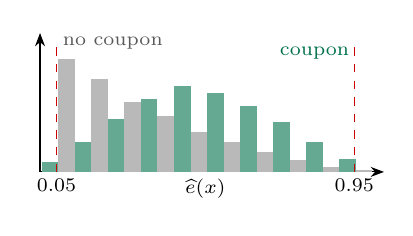
\begin{tikzpicture}[scale=0.42]
% schematic overlap histogram: replace with fig-overlap from the sim
\draw[-{Stealth}] (0,0) -- (10.4,0); \node[font=\scriptsize] at (5,-0.5) {$\widehat e(x)$};
\draw[-{Stealth}] (0,0) -- (0,4.2);
\foreach \x/\h in {0.5/0.3,1.5/0.9,2.5/1.6,3.5/2.2,4.5/2.6,5.5/2.4,6.5/2.0,7.5/1.5,8.5/0.9,9.5/0.4}
  \fill[sbgreen!60] (\x-0.45,0) rectangle (\x+0.05,\h);
\foreach \x/\h in {0.5/3.4,1.5/2.8,2.5/2.1,3.5/1.7,4.5/1.2,5.5/0.9,6.5/0.6,7.5/0.35,8.5/0.15,9.5/0.05}
  \fill[gray!55] (\x+0.05,0) rectangle (\x+0.55,\h);
\draw[dashed, warnred] (0.5,0) -- (0.5,3.8); \draw[dashed, warnred] (9.5,0) -- (9.5,3.8);
\node[font=\scriptsize] at (0.5,-0.4) {0.05}; \node[font=\scriptsize] at (9.5,-0.4) {0.95};
\node[font=\scriptsize, sbgreen] at (8.3,3.6) {coupon}; \node[font=\scriptsize, gray!70!black] at (2.2,3.9) {no coupon};
\end{tikzpicture}\\
{\scriptsize schematic --- replace with the sim's overlap figure}
\end{center}
\end{column}
\end{columns}

\smallskip
Outside the dashed lines one arm is nearly empty. Standardisation \emph{extrapolated} there silently; IPW \textbf{shouts}.
\end{frame}

% ====================================================================
\begin{frame}{Trimming, and Who the Answer Now Describes}

Drop customers with $\widehat e(x)$ outside $[0.05, 0.95]$ --- the bands the rule had all but decided --- and reweight.

\medskip

\begin{center}
\Large $\widehat\tau_{\text{ATT}} = $ \NUM{$+0.16$}{sim coupon-logs v1: Hájek ATT on the trimmed sample} \qquad SE \NUM{0.02}{sim coupon-logs v1: sandwich SE, trimmed} \qquad $\Longrightarrow$ \qquad \textcolor{sbgreen}{\textbf{keep}}
\end{center}

\medskip
\pause

\textbf{The price.} The estimate no longer describes all recipients. It describes the \NUM{91\%}{sim coupon-logs v1: share of treated retained after trimming} of them in bands where the rule left something to chance.

\smallskip

For the top band the logs contain \textbf{no comparison}, and no method manufactures one. The memo says so: \emph{``for the top score band the effect is not identified from Q3 data.''}

\smallskip

Overlap is the warm-up's question in continuous form: \emph{which population are you averaging over?}
\vspace{1.6em}
\end{frame}

% ====================================================================
\begin{frame}{Lin's Table}

\begin{center}
\scriptsize
\begin{tabular}{llrl}
\toprule
\textbf{Method} & \textbf{What it estimates} & \textbf{Lift} & \textbf{Verdict} \\
\midrule
Difference in means & nothing causal & \NUM{$-0.19$}{sim v1: naive} & \textcolor{warnred}{kill} \\
Linear adjustment & variance-weighted average, wrong form & \NUM{$+0.06$}{sim v1: OLS} & \textcolor{warnred}{kill} \\
Flexible standardisation & ATT, extrapolated in the top band & \NUM{$+0.14$}{sim v1: g-formula} & knife edge \\
IPW, untrimmed & ATT, dominated by a few weights & \NUM{$+0.10$}{sim v1: IPW} & \textcolor{warnred}{unclear} \\
IPW, trimmed & ATT on the overlap region & \NUM{$+0.16$}{sim v1: IPW trimmed} & \textcolor{sbgreen}{keep} \\
\midrule
\textit{Truth in the simulation} & ATT & \NUM{$+0.17$}{sim v1: true ATT in the DGP} & \\
\bottomrule
\end{tabular}
\end{center}

\pause

\small Each fails for its own reason, visible only once you ask \textbf{what population} and \textbf{which comparison} it used.
\textbf{Recommendation:} keep the programme in the bands it ran in; do not extend to the top band on this evidence.
\vspace{2.2em}
\end{frame}

% ====================================================================
\begin{frame}{Continuous Dose}

Q4 will vary the face value: \textyen 5, \textyen 10, \textyen 15. The treatment is no longer on/off.

\bigskip

Each customer has a \textbf{curve} of potential outcomes $\{Y(d) : d \in \mathcal{D}\}$; we observe one point on it. Everything today survives with $x$ and $d$ side by side:

\[
\mu(d) \equiv \E[Y(d)] = \E_X\!\bigl[\E[Y \mid D = d, X]\bigr], \qquad
\frac{d\mu}{dd} = \E_X\!\left[\frac{\partial}{\partial d}\E[Y \mid D = d, X]\right]
\]

under exchangeability $\{Y(d)\} \indep D \mid X$ and overlap at every dose.

\bigskip
\pause

What changes:

\begin{itemize}
    \item ``Overlap'' now means every dose observed at every $x$, and a propensity becomes a \emph{density}.
    \item Reporting a whole curve is expensive; reporting its \textbf{slope} is cheap and is usually what the decision needs.
\end{itemize}

\bigskip

\textbf{Next time:} a hotel group whose rates are set by a system, night by night. The treatment is continuous, the rule has 47 inputs, and the question becomes \emph{how} $X$ must enter the model.
\end{frame}

% ====================================================================
\begin{frame}{Key Takeaways}

\begin{itemize}
    \item \spinestep{Estimand.} The CFO's question is the ATT of the programme \emph{as it ran}, held against its own break-even. Extending it to everyone is a different estimand, with a different break-even.
    \item \spinestep{Identification.} The engine's rule is the assignment mechanism. It confounds by construction ($-0.22$ pooled, $+0.17$ within segment). Exchangeability is a claim about the rule, tied to sentences; controls are chosen by timing and cause, not correlation.
    \item \spinestep{Design before analysis.} Reconstruct the rule, check overlap, fix trimming and the estimand, check balance --- all before the outcomes are opened.
    \item \spinestep{Estimation.} Standardisation and IPW are the same identification, seen from the outcome and the assignment side. Where one arm is empty, the first extrapolates silently and the second fails loudly. Report the effective sample size.
    \item \textbf{Every estimate describes a population.} Trimming changes it. Say which.
\end{itemize}

\medskip

\small \textbf{Take-home core:} the Rivergate control audit (30--45 min), due with Notebook 7 --- 96 hours from now. \quad \textbf{Reading:} LaLonde's benchmark --- can observational controls recover an experiment? (Cunningham, \emph{Causal Inference: The Mixtape}, ch.~5; it is also the story behind P3's data.)
\end{frame}

% ====================================================================
\begin{frame}{This Afternoon: Twelve Proposals}

\begin{columns}[T]
\begin{column}{0.36\textwidth}
\small
\begin{tabular}{lr}
\toprule
Talk & 2 min 30 s \\
Feedback & 2 min \\
Transition & 30 s \\
\midrule
Per pair & 5 min \\
Twelve pairs & 60 min \\
\bottomrule
\end{tabular}
\end{column}
\begin{column}{0.60\textwidth}
\small
\textbf{Every proposal must say:}
\begin{enumerate}
    \item \spinestep{Estimand:} who is eligible, what changes, the outcome and horizon, the decision it serves
    \item \spinestep{Identification:} which comparison supplies the missing outcome, and what would make it as good as random
    \item which controls are fixed \emph{before} treatment
    \item \spinestep{Estimation:} the estimator, and where its uncertainty comes from
\end{enumerate}
\end{column}
\end{columns}

\bigskip

\textbf{The room asks one question first:} \emph{What is the comparison group, and what would make it as good as random?}

\bigskip

\small Your revised identification plan is due 48 hours after M8 (72 hours after M10 for IV or panel designs). The design menu lists the assumptions each design needs and the meeting that teaches it.
\end{frame}

\end{document}
